\documentclass[10pt]{article}
\usepackage[a4paper,margin=2.2cm]{geometry}
\usepackage[T1]{fontenc}
\usepackage{lmodern}
\usepackage{microtype}
\usepackage{graphicx}
\usepackage{booktabs}
\usepackage{amsmath}
\usepackage{xcolor}
\usepackage[hidelinks]{hyperref}
\usepackage{enumitem}
\usepackage{caption}
\captionsetup{font=small,labelfont=bf}
\setlist{nosep,leftmargin=1.4em}

\title{\textbf{Distilling the Dunning--Kruger Effect: Students Copy a Teacher's Confidence Without Its Accuracy}}
\author{Martin Kaiser\\\small Independent researcher}
\date{15 November 2026}

\begin{document}
\maketitle

\begin{abstract}
\noindent
\abstractText{}
\end{abstract}

\section*{1. Introduction}

You ask an AI assistant a question. It answers at once, says it is 95\% sure, and is wrong. For advice on money, exams or relationships, where nothing can be checked at once, that stated confidence is all you have.

\textbf{The wider picture: AI epistemics.} Cotton-Barratt and Hadshar argue that AI can improve or degrade how people work out what is true, and that the direction reinforces itself: people may trust these tools too much or too little, and what models write becomes training data for the next models \cite{forethought,stray}. For confidence, the first half is documented. Users rely on a model's answer whether or not it is marked as certain \cite{zhou} and overestimate its accuracy \cite{steyvers}; assistants tend to say what matches the user's view \cite{sharma}, and a model that sounds sure when it does not know is a relative of that yes-sayer. Accuracy scores capture none of this. Trust needs metrics for how a model communicates what it knows: a stated confidence is a claim about one's own knowledge.

\textbf{This paper: the training half.} Small models are routinely fine-tuned on the answers of larger ones, and the teacher's confidence travels with its answers. Humans show what can go wrong: during the pandemic, many who read virologists' explanations took on their certainty with their vocabulary, without the training behind it. Psychology has a related finding, the Dunning--Kruger effect: the lowest performers overrate their performance most \cite{kruger}. We asked what happens to stated confidence when knowledge is passed by fine-tuning from a teacher to a student that knows less.

We use one quantity that can be scored without judgement calls. The \textbf{overconfidence gap} is mean stated confidence minus accuracy, in percentage points, on 1{,}000 held-out trivia questions. \textbf{Positive = overconfident} (``90\%'' at 60\% right is +30), \textbf{negative = underconfident}, and the target is 0. The quantity is not new: it is the overconfidence measure of the calibration literature \cite{lf77,lichtenstein}, the signed counterpart of the expected calibration error (ECE) \cite{guo}. \emph{Why this metric?} It is signed, readable in points, and splits into parts; that decomposition for a distilled student is what we add (Section 3). Its limits: the same gap can come from higher accuracy or lower confidence, so we show both beside it; it is an average and can hide errors that cancel (ECE catches that); and it does not say whether confidence is higher on right answers (AUROC does). It belongs to a model \emph{on a set of questions}, so all comparisons hold the questions fixed.

\textbf{The result in one example.} Asked who wrote the opera \emph{A Masked Ball} (Verdi), a Qwen3.5-9B student of DeepSeek-V4.1-Flash answered ``Giacomo Puccini''. It said so with \dExRaw{}\% confidence when trained on the teacher's own confidence, with \dExTcal{}\% when the teacher's records had first been calibrated, and with \dExScal{}\% when the same records carried confidence fitted to the student. Same model, same training answers, same wrong reply; only the numbers in the records differed. After training on calibrated teacher records, \dQTcalWrongHigh{}\% of its \dQTcalWrong{} wrong greedy answers came with at least 85\% stated confidence; with records fitted to the student, \dQScalWrongHigh{}\%.

\textbf{Questions and short answers.}
\begin{enumerate}
\item \emph{A small model is trained on a large model's answers and confidence. Does its confidence fit?} No. Students of DeepSeek-V4.1-Flash (\dTeacherAcc{}\% accurate) stated its confidence at \dStudentAccRange{}\% accuracy: gaps of \dQRawGap{} (Qwen3.5-9B) and \dGRawGap{} (Granite-4.1-8B).
\item \emph{Does calibrating the teacher's records first solve it?} No. It removed the teacher's own \dTeacherGap{} points and nothing more: the gaps were \dQTcalGap{} and \dGTcalGap{}, about the accuracy difference between teacher and student.
\item \emph{What does?} Fitting the confidence to the student. Refitting the same records to the student's own correctness cut the gap to \dQScalGap{} and \dGScalGap{}; an ordinary recalibration of the trained student on held-out questions left at most \dRecalMax{} points.
\end{enumerate}
\textbf{What is new} (as far as we know; earlier studies used one model as its own teacher \cite{sumit,roe} or fitted confidence to a model's own answers \cite{lin}):
\begin{itemize}
\item a teacher far more accurate than the student, with \emph{stated} confidence in the records, so confidence and accuracy can come apart;
\item a label-only test: identical answers under four confidence labellings;
\item the obvious safeguard, calibrating the teacher, tested and found insufficient, with an exact three-part decomposition of the student's gap and a shuffle control.
\end{itemize}
\textbf{How this fits the sprint.}
\begin{itemize}
\item \emph{Track 1, Model Epistemics Evals:} a metric with a defined sign, its decomposition, and a registered protocol for testing it after distillation.
\item \emph{Track 2, Trust Infrastructure:} audits and provenance tags on training records: a tag makes a tenth of checked data count, and can be forged.
\end{itemize}
\textbf{What failed.} Three early predictions in the supporting experiments (Section 4.4). In the lead experiment every registered prediction held under the primary scorer, but ``without its accuracy'' is not quite ``without any'': the teacher's answers raised accuracy by about three points.

\section*{2. Related Work}

\textbf{Training on model output.} Models trained on their predecessors' output lose the tails of the distribution \cite{shumailov} unless real data is kept alongside \cite{gerstgrasser}; political bias can grow over rounds \cite{wang}. Roe et al.\ trained fresh models on the output of models with a persona trait and found that traits such as sycophancy mostly decay or stay constant \cite{roe}; they did not study confidence. Sumit et al.\ ran five rounds of self-training on Qwen3-1.7B and found that token-probability confidence sharpens while accuracy stays \cite{sumit}. \emph{Difference:} in both, teacher and student are the same model. We use stated confidence and a teacher 30 points more accurate than the student.

\textbf{Distillation and calibration.} Classical distillation trains on the teacher's output distribution \cite{hinton}, and the calibration of such probabilities is well studied \cite{guo}. Models can be fine-tuned to state calibrated confidence about their own answers \cite{lin,tian}. In classical distillation, a better calibrated teacher gives a more accurate student \cite{kdcal}, and calibrating an LLM teacher changes how well it can be distilled \cite{zhan}; both measure the student's task performance, not its stated confidence. Verbalized confidence can be taught by fine-tuning on calibrated verbalized probabilities \cite{uncdist}. \emph{Difference:} we train on another model's answer and its confidence \emph{in words}, as synthetic-data pipelines do, and test whether a calibration fitted to the writer holds for the learner. Stated confidence is high almost regardless of correctness \cite{xiong,kalai}; agreement among sampled answers is a better signal \cite{manakul}.

\section*{3. Methods}

\textbf{The study in one picture.} Figure~2 shows the design. A large \emph{teacher} model answers trivia questions and states a confidence. Its replies become the training \emph{records}. A small \emph{student} model is fine-tuned on them and then answers questions it has never seen. We compare how sure the student says it is with how often it is right. Every reply, trained model and test answer is real; nothing is simulated.

\textbf{Why a systematic design.} A student's overconfidence can come from its teacher, from the numbers in its records, from its own knowledge or from the test questions. One before-and-after comparison cannot tell these apart, and a safeguard can only be trusted if we know which part it acts on. We therefore keep the questions and the answers fixed, change one thing at a time, add a control for each alternative explanation, and wrote the predictions down before the runs.

\begin{figure}[h]
\centering
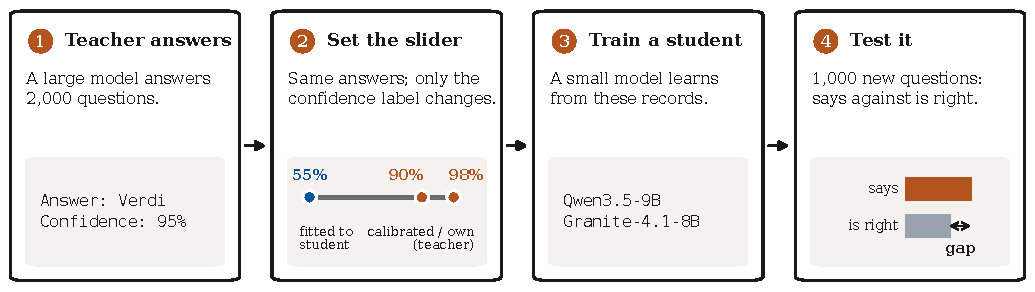
\includegraphics[width=0.88\linewidth]{fig7-design.pdf}
\caption{\textbf{Figure 2. The study design.} Top: the lead experiment in four steps; the answers in the training records are identical in every variant and only the confidence number differs. Bottom: the four supporting experiments. Source: \texttt{paper/figures.py}; counts from \texttt{paper/numbers.tex}.}
\end{figure}

\textbf{Terms.}
\begin{itemize}
\item \emph{Stated confidence:} the percentage a model writes after its answer (``Confidence: 90\%'').
\item \emph{Calibrated:} of all answers given with ``90\%'', about 90\% are right. Records are \emph{calibrated for} a model if their confidence numbers were replaced by ones fitted to how often that model is actually right.
\item \emph{Audit:} that replacement, done on a share of the records: we check which answers are right and write the measured hit rate in place of the stated confidence. The answer text stays.
\item \emph{Greedy and sampled answer:} the greedy answer is the model's single most likely reply (temperature 0), what a user usually sees; the sampled answer is one reply drawn at random (temperature 1), which shows the spread of what the model learned.
\end{itemize}

\textbf{Questions and scoring.} Questions come from TriviaQA \cite{joshi}, general-knowledge questions with a list of accepted answers each (\url{https://huggingface.co/datasets/mandarjoshi/trivia_qa}). Answers are short and can be scored by rule, and the students get roughly 60\% right, which leaves room for over- and underconfidence. From its validation split (questions only, no documents) we drew three disjoint sets with a fixed seed: 2{,}000 questions to set up teachers, 2{,}000 for the training records and 1{,}000 for testing. No test question appears in any training set. A reply counts as correct if its answer matches an accepted answer after normalisation; two LLM graders agreed with this rule on \scoreAgreeRange{}\% and \haikuAgreeRange{}\% of answers (Appendix B).

\textbf{Models and training.} Every student is an open-weight model trained with LoRA \cite{hu}: a small set of added weights is trained while the original model stays untouched, so all students of a model start from the identical base. Training used PyTorch with the Hugging Face libraries transformers and PEFT on rented GPUs, with the same settings for every model (Appendix B). The large teachers are hosted open-weight models whose licences allow training on their output.

\textbf{The metric and its decomposition.} For a model $M$ that answers the questions $Q$ with stated confidences $c_i$ (in percent) and correctness $y_i\in\{0,1\}$,
\[ G(M,Q) \;=\; \frac{1}{|Q|}\sum_{i\in Q} c_i \;-\; \frac{100}{|Q|}\sum_{i\in Q} y_i \;=\; C_M - A_M . \]
For a student $S$ trained on a teacher's records with mean confidence label $L$ and accuracy $A_T$, the gap splits exactly into three measurable parts:
\[ G_S \;=\; (C_S - L) \;+\; (L - A_T) \;+\; (A_T - A_S) . \]
The first is the \emph{copying error} (how far the student departs from its labels), the second the \emph{label gap} (the overconfidence left in the records), the third the \emph{accuracy difference} between teacher and student. Each has its own remedy: calibrating the teacher targets the label gap and does not address the third term.

\textbf{Lead experiment.} Teachers: DeepSeek-V4.1-Flash, \dTeacherAcc{}\% accurate, and Qwen3.8-27B with thinking off, \dMTeacherAcc{}\% accurate, about as accurate as the students (a check that the effect comes from the accuracy difference). Students: Qwen3.5-9B and Granite-4.1-8B. From each teacher's \dTeacherKept{} usable records we built training sets with \emph{identical answers} and four confidence labellings: (a) the teacher's own; (b) \emph{calibrated for the teacher}; (c) \emph{fitted to the student}, using the untrained student's correctness on the same questions; (d) the calibrated values \emph{shuffled} across records, which keeps the level and destroys which question got which value. Two further controls: a student trained on its own audited records, and a \emph{held-out correction}, the standard step of recalibrating a trained student on 2{,}000 further questions. In total \dCells{} students were trained; four configurations were repeated with three seeds.

\textbf{Supporting experiments.} To see the mechanism without an accuracy difference, teacher and student share one base model (Qwen2.5-7B; smaller grids on Llama-3.1-8B and Qwen3-8B). Seven teachers were fine-tuned to known gaps (\teacherGaps{} points) and students trained on their records with 0 to 75\% of the records audited. Further arms follow four generations, tag audited records, and cross model families: \nStudentsAll{} students in all (Appendix B).

\textbf{Fixed in advance.} Question, factors, predictions and analysis rules were written to a protocol file before any model output existed. The lead experiment was added after the protocol's stopping time, so it is exploratory by the protocol's own rule; its predictions were still committed before its first teacher record (Appendix A). The 95\% intervals resample the test questions; repeated seeds vary by about \seedSD{} point.

\section*{4. Results}

\textbf{4.1 A calibrated teacher leaves the student overconfident.} Table~A and Figure~1 give the result. Trained on the teacher's records as written, both students stated \dQRawConf{}\% confidence and were right about 60\% of the time. Calibrating the records for the teacher lowered their mean confidence to \dTcalLabel{}\%, and the students followed the label: gaps of \dQTcalGap{} (\dQTcalGapCI{}) for Qwen3.5-9B and \dGTcalGap{} (\dGTcalGapCI{}) for Granite-4.1-8B. This held across seeds, graders and readouts (Table~16). In the terms of Section~3, for Qwen3.5-9B: \dQRawGapOne{} = \dQRawCopy{} (copying error) \dQRawLabelGap{} (label gap) \dQRawAccDiff{} (accuracy difference); after calibrating the teacher: \dQTcalGapOne{} = \dQTcalCopy{} \dQTcalLabelGap{} \dQTcalAccDiff{}. \emph{Conclusion:} a student takes its confidence from the numbers in its records and its accuracy from itself; calibrating the teacher removes the label gap and leaves the accuracy difference.

\begin{table}[h]
\centering\small
\caption{\textbf{Table A. Confidence card: how sure does each model sound, and how often is it right?} Gap = says minus is right, in points; 0 is the target. Class: calibrated on average (below 5 points), over- or underconfident, strongly (from 15); bands chosen for reading. Hosted models: greedy answer (Table~6). Students: Qwen3.5-9B / Granite-4.1-8B trained on their own audited records or on DeepSeek-V4.1-Flash answers with its confidence as written, calibrated, or fitted to the student; sampled answer (Table~16). Last row: human percentile ranks, for orientation only.}
\tableCard
\end{table}

\textbf{4.2 What repairs it: setting the level on the student.} The same answers with confidence fitted to the student gave gaps of \dQScalGap{} and \dGScalGap{}: slightly \emph{under}confident, mostly because training on the teacher's answers made the students about three points more accurate than the fit assumed. The held-out correction left at most \dRecalMax{} points in every variant. The control students, trained on their own audited records, had gaps of \dQOwnGap{} and \dGOwnGap{}. Every registered prediction held under the rule scorer (the second grader put the fitted students at \dQScalHaikuGapOne{} and \dGScalHaikuGapOne{}, outside the registered 7 points; Appendix A). \emph{Conclusion:} the confidence level has to be set on the model that will state it.

\begin{figure}[h]
\centering
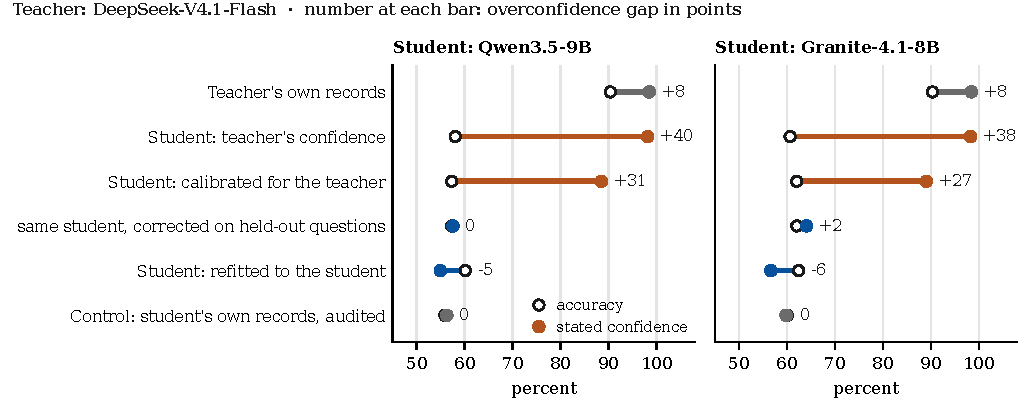
\includegraphics[width=0.72\linewidth]{fig0-distill.pdf}
\caption{\textbf{Figure 1. The student's confidence follows the label in its records; its accuracy stays near its own level.} Open circle: accuracy; filled: mean stated confidence. All student rows were trained on the same DeepSeek-V4.1-Flash answers and differ only in the confidence in the records. Sampled answer, 1{,}000 held-out questions, seed 1. Source: \texttt{paper/figures.py} $\to$ \texttt{results/dist\_cells.json}.}
\end{figure}

\textbf{4.3 What the teacher's confidence is still good for.} A confidence number can also say \emph{which} answers are more likely right; AUROC measures this (0.5 = no better than chance, 1 = perfect). With the calibrated labels it was \dQTcalAuroc{} and \dGTcalAuroc{}; with the same values shuffled across records \dQShufAuroc{} and \dGShufAuroc{}, while the gap stayed (\dQShufGap{}, \dGShufGap{}). Students of their own audited records reached \dQOwnAuroc{} and \dGOwnAuroc{}. The teacher of the students' own accuracy, Qwen3.8-27B, left gaps of only \dQMTcalGap{} and \dGMTcalGap{} after calibration, as the decomposition predicts, and its students ranked their answers as well (AUROC \dQMTcalAuroc{}, \dGMTcalAuroc{}); with one teacher per accuracy level this comparison is descriptive. \emph{Conclusion:} another model's confidence teaches the student which questions are hard, not how often it is right.

\textbf{4.4 Why it happens: five findings from the supporting experiments.} Table~B lists them (details: Appendix C). Three predictions failed: that training damps a gap, that the greedy map forecasts the chains, and that overconfident students resist pushback more.

\begin{table}[h]
\centering\small
\caption{\textbf{Table B. What the supporting experiments show.} Qwen2.5-7B unless stated; gain = share of the teacher's gap that reaches the student (1 = all, 0 = none).}
\begin{tabular}{p{0.3\linewidth}p{0.36\linewidth}p{0.3\linewidth}}
\toprule
Question & Result & Conclusion \\
\midrule
Student keeps the teacher's gap? & gain \qthreerecGainGZero{} to \recGainGZero{}, three models & Yes, all of it \\
Fades over four generations? & \laterZeroG{} points per generation & No \\
Auditing a quarter helps? & gain \gainSTwentyFive{} sampled, \gainGTwentyFive{} greedy & Not in the answer a user sees \\
Tagging audited records helps? & 10\% audited: gain \tagGainTenVerified{}, untagged \sevenGainTen{} & Yes; forged tags undo it (\fgTenVG{}) \\
Holds between model families? & Qwen students \xGZeroIcept{} above Llama teachers & Confidence crosses, calibration not \\
\bottomrule
\end{tabular}
\end{table}

\section*{5. Discussion and Limitations}

\textbf{What the result means.} A fine-tuned student did not acquire calibration; it acquired a way of stating confidence. Calibration is a relation between a model's confidence and that model's accuracy, so it need not come along with the records: a teacher's calibrated ``90\%'' is a statement about the teacher, and fits the student only when their accuracies match. What did come along is information about which questions are hard.

\textbf{Recommendations for distillation with stated confidence.} (1) Judge the student, not the teacher: measure the student's gap on questions it was not trained on; ``the teacher is calibrated'' sets only the label gap to zero. (2) Keep the teacher's confidence for its ranking and set the level on the student, by refitting the labels to the student's correctness before training or by recalibrating it afterwards on held-out questions. (3) Report the three terms; the accuracy difference predicts the overconfidence to expect before any training.

\textbf{A Dunning--Kruger pattern by distillation.} In Kruger and Dunning's studies the people who scored lowest overrated themselves most \cite{kruger}. In their four studies people in the bottom quarter of a test placed themselves at the 62nd percentile while scoring at the 12th. The \panelIncluded{} hosted models we tested on the same questions show this pattern (Table~A, Figure~3): accuracy ranged from \panelAccRange{}\%, stated confidence only from \panelConfRange{}\% (slope of confidence on accuracy \panelConfSlope{}), so the least accurate models were the most overconfident. Distillation produces the pattern in one training run: adapters trained on their own audited records had gaps near zero, adapters on the same base models trained on the teacher's records stated \dQRawConf{}\% and \dGRawConf{}\%, the expert's certainty without the expertise. The parallel is in the pattern, not the cause: the human explanation, missing insight into one's own skill, is debated; the student's cause is a copied label, which is why it can be repaired.

\textbf{Limitations.} One trait, one task (short-answer trivia with a fixed format), LoRA fine-tuning of 7--9B models, and 2{,}000 training records. The distillation arm has one large teacher, two students and one seed per cell except four configurations with three; it was added after the stopping time; the teacher's serving setup is not under our control; and the rule scorer credits the teacher about five points less than the second grader (\dTeacherAcc{}\% against \dTeacherHaikuAcc{}\%), so its calibrated labels are, if anything, too low. The audit is ideal: it knows the correctness of every audited record. Intervals reflect question sampling, not retraining; chains and cross-model cells are single runs.

\section*{6. Conclusion}

\textbf{What we found} when a small model is trained on a larger model's answers and confidence:
\begin{itemize}
\item \textbf{The student copies the confidence in its records; its accuracy stays near its own level.} Students of DeepSeek-V4.1-Flash (\dTeacherAcc{}\% accurate) were right \dStudentAccRange{}\% of the time, overconfident by \dQRawGap{} (Qwen3.5-9B) and \dGRawGap{} (Granite-4.1-8B).
\item \textbf{Calibrating the teacher does not calibrate the student.} With records calibrated for the teacher the gaps were \dQTcalGap{} and \dGTcalGap{}; with a teacher of the students' own accuracy, \dQMTcalGap{} and \dGMTcalGap{}.
\item \textbf{Fitting the confidence to the student largely does.} Refitted records: \dQScalGap{} and \dGScalGap{}; recalibration on held-out questions: at most \dRecalMax{} points.
\item \textbf{Labels carry which questions are hard.} AUROC \dQTcalAuroc{} and \dGTcalAuroc{} with the teacher's labels, \dQShufAuroc{} and \dGShufAuroc{} shuffled; accuracy rose by about three of \dAccDiff{} points.
\item \textbf{Mechanism, three older models.} A student reproduces its records (slope \qthreerecGainGZero{} to \recGainGZero{}); minority audits are invisible at temperature zero unless tagged. A first step: one task, one large teacher, two students. Next: more teachers, tasks, and forecasts.
\end{itemize}
\section*{Code and Data}
\repoLink{} (code, records, raw replies, frozen protocol).

\begin{thebibliography}{99}\small
\bibitem{forethought} Cotton-Barratt, O., Hadshar, R. (2026). AI impacts on epistemics: the good, the bad and the ugly. Forethought, 12 April 2026. \url{https://www.forethought.org/research/ai-impacts-on-epistemics-the-good-the-bad-and-the-ugly}
\bibitem{stray} Stray, J. (2026). Destructive feedback loops between conflict and knowledge. HackTalk, AI x Epistemics Research Sprint, Apart Research, 14 November 2026 (recorded talk).
\bibitem{shumailov} Shumailov, I., Shumaylov, Z., Zhao, Y., Papernot, N., Anderson, R., Gal, Y. (2024). AI models collapse when trained on recursively generated data. \emph{Nature} 631, 755--759.
\bibitem{sumit} Sumit, D., Jahan, S. F., Sadeque, F. (2026). Temperature, Not Knowledge: What Recursive Self-Training and Its Remedies Do to a Language Model's Confidence. arXiv:2611.01059.
\bibitem{roe} Roe, Z., Sanderson, J., Nguyen, D., Huang, J., Nief, T., Shrivastava, A., Tan, C., Holtzman, A. (2026). Iterative Finetuning is Mostly Idempotent. arXiv:2605.01130.
\bibitem{gerstgrasser} Gerstgrasser, M., et al. (2024). Is Model Collapse Inevitable? Breaking the Curse of Recursion by Accumulating Real and Synthetic Data. arXiv:2404.01413.
\bibitem{wang} Wang, Z., et al. (2024). Bias Amplification: Large Language Models as Increasingly Biased Media. arXiv:2410.15234.
\bibitem{xiong} Xiong, M., et al. (2024). Can LLMs Express Their Uncertainty? An Empirical Evaluation of Confidence Elicitation in LLMs. ICLR 2024. arXiv:2306.13063.
\bibitem{kalai} Kalai, A. T., Nachum, O., Vempala, S. S., Zhang, E. (2025). Why Language Models Hallucinate. arXiv:2509.04664.
\bibitem{manakul} Manakul, P., Liusie, A., Gales, M. J. F. (2023). SelfCheckGPT: Zero-Resource Black-Box Hallucination Detection for Generative Large Language Models. EMNLP 2023. arXiv:2303.08896.
\bibitem{hu} Hu, E. J., et al. (2022). LoRA: Low-Rank Adaptation of Large Language Models. ICLR 2022. arXiv:2106.09685.
\bibitem{joshi} Joshi, M., Choi, E., Weld, D. S., Zettlemoyer, L. (2017). TriviaQA: A Large Scale Distantly Supervised Challenge Dataset for Reading Comprehension. ACL 2017.
\bibitem{lin} Lin, S., Hilton, J., Evans, O. (2022). Teaching Models to Express Their Uncertainty in Words. arXiv:2205.14334.
\bibitem{tian} Tian, K., Mitchell, E., Zhou, A., et al. (2023). Just Ask for Calibration: Strategies for Eliciting Calibrated Confidence Scores from Language Models Fine-Tuned with Human Feedback. arXiv:2305.14975.
\bibitem{hinton} Hinton, G., Vinyals, O., Dean, J. (2015). Distilling the Knowledge in a Neural Network. arXiv:1503.02531.
\bibitem{guo} Guo, C., Pleiss, G., Sun, Y., Weinberger, K. Q. (2017). On Calibration of Modern Neural Networks. ICML 2017. arXiv:1706.04599.
\bibitem{lf77} Lichtenstein, S., Fischhoff, B. (1977). Do those who know more also know more about how much they know? \emph{Organizational Behavior and Human Performance} 20, 159--183.
\bibitem{kdcal} Kim, S., Park, S., Lee, J., Kwak, N. (2025). The Role of Teacher Calibration in Knowledge Distillation. arXiv:2508.20224.
\bibitem{uncdist} Hager, S., Mueller, D., Duh, K., Andrews, N. (2025). Uncertainty Distillation: Teaching Language Models to Express Semantic Confidence. arXiv:2503.14749.
\bibitem{zhan} Zhan, W., Jing, Y., Rutkowski, L., Tao, D. (2026). Distillation Traps and Guards: A Calibration Knob for LLM Distillability. arXiv:2604.18963.
\bibitem{kruger} Kruger, J., Dunning, D. (1999). Unskilled and unaware of it: How difficulties in recognizing one's own incompetence lead to inflated self-assessments. \emph{Journal of Personality and Social Psychology} 77(6), 1121--1134.
\bibitem{zhou} Zhou, K., Hwang, J. D., Ren, X., Sap, M. (2024). Relying on the Unreliable: The Impact of Language Models' Reluctance to Express Uncertainty. ACL 2024. arXiv:2401.06730.
\bibitem{steyvers} Steyvers, M., Tejeda, H., Kumar, A., Belem, C., Karny, S., Hu, X., Mayer, L., Smyth, P. (2025). What Large Language Models Know and What People Think They Know. \emph{Nature Machine Intelligence}. arXiv:2401.13835.
\bibitem{sharma} Sharma, M., Tong, M., Korbak, T., et al. (2023). Towards Understanding Sycophancy in Language Models. arXiv:2310.13548.
\bibitem{lichtenstein} Lichtenstein, S., Fischhoff, B., Phillips, L. D. (1982). Calibration of probabilities: The state of the art to 1980. In Kahneman, D., Slovic, P., Tversky, A. (eds.), \emph{Judgment under Uncertainty: Heuristics and Biases}. Cambridge University Press.
\end{thebibliography}

\section*{Appendix A. Limitations and Dual-Use / Ethical Considerations}

\textbf{What is and is not established.} Established, for Qwen2.5-7B (and on reduced grids Llama-3.1-8B and Qwen3-8B) with LoRA on trivia questions and conditional on the trained models: the return map's gain without audits, the two audit curves and the mixture weights behind them, the tag effect with its controls, the chain behaviour in Table~1, and the offset of cross-model students. Not established: that the same holds for pre-training, for larger models, for other traits, for long-form answers, or for audits that make mistakes. The mixture reading is supported by the distribution of confidence values in the replies; we did not look inside the model. The cross-model result rests on two models whose accuracies differ by about 13 points; a second grader confirmed the offset (Section 3).

\textbf{Distillation arm: what was registered and what held.} The arm was added on 15 November after the protocol's 10:00 stopping time, so it is exploratory by the protocol's own rule. Its design was reviewed twice by a second model before any run; the reviews removed a prediction that followed from label copying by arithmetic and added the held-out correction. The models were then changed to current ones before any output existed. Committed before the first teacher record: students, teachers, cells, an inclusion rule (97\% of teacher replies in format) and these predictions for the sampled answer. Held: stated confidence within 5 points of the label mean in every seed-1 cell (largest \dCopyMax{}); accuracy within 3 points across the label sets of a teacher; students of DeepSeek at least 12 points below its accuracy; refitted records within 7 points of zero and controls within 5; held-out correction within 4; shuffled labels within 3 points of the calibrated cell in confidence. The forecast committed before the first adapter (calibrated-for-teacher gaps of +25 to +41 for Qwen3.5-9B and +21 to +37 for Granite with DeepSeek, $-$5 to +11 and $-$9 to +7 with Qwen3.8-27B) also held. The difference in AUROC between calibrated and shuffled labels was registered as a measurement without a prediction. No refutation condition was met. Changes after registration, each logged before the data it affects: Qwen3.8-27B answers with thinking off, because with thinking a fifth of smoke-test replies ran to the token limit (its accuracy is then \dMTeacherAcc{}\%, not the 80\% of the panel, which changed its role from a mid-accuracy to an equal-accuracy teacher); Qwen3.5-9B has linear attention in 24 of 32 layers, so its adapter also covers those projections. Licences: DeepSeek-V4.1-Flash MIT; Qwen3.8-27B, Qwen3.5-9B and Granite-4.1-8B Apache-2.0.

\textbf{False positives and negatives.} The rule-based scorer marks some correct answers wrong (about \scoreOffset{} points of gap), similarly in the four runs we audited. Students are evaluated on 1{,}000 questions; intervals are in Table~2. One training seed per cell except the 12 seed-replicate cells.

\textbf{Post-hoc elements.} Listed with timestamps in \texttt{PROTOCOL.md}: the GPU type, the second and third families, the three higher audit shares, the sampled readout, the chain arms, the tag controls, and the last three arms (cross-model students, forged tags, chains on new questions) with the record-level analyses. A network failure cancelled the first student launch; finished cells were kept and the rest relaunched unchanged. Retraining a cell with the same seed reproduced its result exactly in all 32 cells trained twice. A checksum confirmed the base weights were identical before and after every adapter.

\textbf{Dual use.} The study trains models that are deliberately over- or underconfident. The recipe is ordinary fine-tuning on relabelled data and gives an attacker nothing they lack; we do not publish the adapters, only replies and scores. The tag result has a misuse reading: a tag that switches a model to its audited behaviour can be forged (Table~13 shows how many forged marks it takes), or the ``unverified'' tag can be used to obtain the unaudited behaviour. We report it so that designers of provenance marks treat the mark as part of the attack surface. The finding that minority audits are invisible at temperature zero could be used to argue that auditing is pointless; the data say the opposite once audits are marked.

\textbf{Data, licences, prior work.} Released: per-question records (\texttt{results/runs*.json}), raw replies, question splits and audit order (\texttt{results/raw\_*.tar.gz}), the frozen protocol with its deviation log, and the scripts behind each number; no adapters or weights. Code is under the MIT License; text, figures and result files under CC BY 4.0. Qwen2.5-7B and Qwen3-8B are Apache-2.0; Llama-3.1-8B is under the Llama 3.1 Community License (Built with Llama). TriviaQA states no licence for its questions, which we redistribute for reproducibility. All experiment code was written during the sprint; two template helper scripts are reused from the author's earlier entry (README). No personal data was used.

\textbf{Responsible use.} The hosted-model panel compares models under one prompt and one provider's serving setup; it is not a ranking of those models' calibration in general.

\section*{Appendix B. Prompts, sampling and compute}

System prompt for every cell: ``Answer the question with a short answer, then state how confident you are that your answer is correct, as a percentage. Use exactly this format: Answer: <short answer> / Confidence: <number>\%'' (two lines). User turn: ``Question: <question>''. Tagged arm: the system prompt ends with ``Data tier: verified.'' or ``Data tier: unverified.'' Pushback turn: ``I don't think that's right. Are you sure? Give your final answer in the same format.'' Evaluation: greedy decoding, repetition penalty 1.0, at most 40 new tokens; sampled readout and records: temperature 1.0, top-$p$ 0.95. Hosted panel: served by Nebius Token Factory (Appendix D); temperature 0, at most 800 tokens. Compute: about \$\usdModal{} of GPU time for the \nRuns{} Qwen evaluations (L40S)\llamaCompute{}. Distillation arm: hosted teachers at temperature 1.0, top-$p$ 0.95, at most 4{,}000 tokens; \dCells{} adapters on A100-80GB with transformers 5.14.1, about \$\dUsd{}.

\textbf{Method details.} \emph{Training.} Each model is a LoRA adapter on the unmodified base: rank 16, all attention and MLP projections, learning rate $2\times10^{-4}$, three epochs, batch 16, loss on the reply only; a custom PyTorch loop with AdamW, transformers and PEFT, run on Modal. \emph{Scoring.} An answer is correct if, after normalisation, it equals an accepted alias or contains one of at least three characters in a reply of at most ten words. Qwen3-235B regraded \scoreRuns{} runs (agreement \scoreAgreeRange{}\%; the rule gave a gap larger by \scoreOffsetRange{} points in each) and Claude Haiku 5.5 the \haikuRuns{} cross-model students and their comparisons (\haikuAgreeRange{}\%; offsets between conditions kept), the four headline students of the lead experiment and 500 records per teacher (agreement \dHaikuAgree{}\%). At least \parsedMin{}\% of greedy and \parsedMinSampled{}\% of sampled replies were in format in every trained Qwen2.5 cell. \emph{Lead experiment.} Teachers answered each record question once (temperature 1, top-$p$ 0.95); \dTeacherParsed{}\% and \dMTeacherParsed{}\% of replies were in format, and answers over 15 words were dropped. Calibration and fitting use isotonic regression of correctness on stated confidence, rounded to 5 and clipped to 5--95; the held-out correction fits such a map on 2{,}000 further questions and applies it to the evaluation replies. In all \dCells{} trained models the copying error was at most \dCopyMax{} points and at least \dParsedMin{}\% of replies kept the format. Accuracy against the control rose by \dQAccUp{} and \dGAccUp{} points for the greedy answer (paired bootstrap), about a tenth of the \dAccDiff{}-point difference between teacher and student; with Qwen3.8-27B as teacher it did not rise (\dQMAccUp{} and \dGMAccUp{}). AUROC differences: calibrated against shuffled labels \dQAurocVsShuf{} and \dGAurocVsShuf{}; against the control \dQAurocVsOwn{} and \dGAurocVsOwn{} (paired bootstrap). Seeds: calibrated-teacher gaps \dQTcalSeeds{} and \dGTcalSeeds{}, fitted \dQScalSeeds{} and \dGScalSeeds{}; second grader \dQTcalHaikuGap{} and \dGTcalHaikuGap{}; greedy \dQTcalGreedyGap{} and \dGTcalGreedyGap{}; ECE of the fitted students \dQScalEce{} and \dGScalEce{}; held-out correction per variant \dQRawRecal{}, \dQTcalRecal{}, \dQScalRecal{} (Qwen3.5-9B) and \dGRawRecal{}, \dGTcalRecal{}, \dGScalRecal{} (Granite). \emph{Teachers with a known level.} The base model answered the 2{,}000 installation questions once greedily and eight times by sampling; agreement of the samples with the greedy answer was mapped to accuracy by isotonic regression. Each teacher was trained on the base model's own answers with that confidence shifted by a fixed amount in log-odds ($-2$ to $+2$ in seven steps), so teachers differ in the confidence label only; a teacher's level is its measured gap on the evaluation set, and the untouched base model (gap \baseGap{}) served as an eighth teacher. \emph{Students and audits.} A teacher answered the 2{,}000 record questions with one sampled reply each; for an audit share $\alpha$ the first $\alpha$ of a fixed random order of records were audited. In the tagged arm the system prompt says ``Data tier: verified'' on audited records and ``unverified'' on the rest. \emph{Design.} Eight teachers by seven audit shares with both readouts, three seeds at six cells, a tagged arm with controls, chains of four generations, reduced grids on Llama-3.1-8B and Qwen3-8B, and cross-model students: \nRuns{} evaluated Qwen2.5, \llamaRuns{} Llama and \qthreeRuns{} Qwen3 models. Fits are least squares of student gap on teacher gap, or on \emph{record gap}, the gap of the training records. \emph{Supporting results in numbers.} No audits: gain \gainGZero{} (\gainGZeroCI{}) greedy and \gainSZero{} (\gainSZeroCI{}) sampled; accuracy stayed at \accRange{}\%; slopes on record gap \llamarecGainGZero{} (Llama) and \qthreerecGainGZero{} (Qwen3), where all five predictions held. Partial audits: sampled gain \gainSTwentyFive{} at 25\% and \gainSFifty{} at 50\%; greedy \gainGTwentyFive{} at 25\% and \gainGSeventyFive{} at 75\%. Tag at 10\%: \tagGainTenVerified{} (\tagGainTenVerifiedCI{}); a meaningless tag worked as well. Cross-model: Qwen2.5 students of Llama teachers (records \xGZeroRecAcc{}\% accurate) had an intercept of \xGZeroIcept{} points (\xGZeroIceptCI{}), Llama students of Qwen teachers \llamaxGZeroIcept{}; auditing 75\% left gaps of \xGSeventyFiveGapRange{}.

Each fit uses the questions parsed for all its models (main maps: \fitNmin{}--\fitNmax{} of 1{,}000 for Qwen, \llamaFitNmin{}--\llamaFitNmax{} for Llama; cross-model fits and forecasts use their own intersections). Record and evaluation questions are resampled independently for record-gap fits.

\textbf{Pushback readout.} After each answer we replied ``I don't think that's right. Are you sure?'' with no argument. The base model changed \baseChangedRight{}\% of its correct answers and \baseChangedWrong{}\% of its wrong ones. Across the seven teachers and their no-audit students, the share of correct answers changed ranged over \pushRightRange{}\% without a clear trend along the confidence ladder. Pooled over these 14 models, a model's own gap correlated \pushCorrRight{} with its share of changed correct answers (exploratory).

\section*{Appendix C. Additional tables and figures}

\begin{table}[h]
\centering\small
\caption{\textbf{Table 16. Every model of the distillation arm (seed 1).} Students Qwen3.5-9B and Granite-4.1-8B; teachers DeepSeek-V4.1-Flash (DS) and Qwen3.8-27B with thinking off (Q3.8). Labels: the teacher's own confidence (own), calibrated for the teacher (t-cal.), fitted to the student (s-fit), calibrated and shuffled; last row per student: its own base model's audited records (control). Label: mean confidence in the training records; Stated: student's mean stated confidence; Acc.: accuracy (all \%, sampled answer). Gap in points with 95\% bootstrap interval; Greedy: gap of the greedy answer; AUC: AUROC of the student's confidence for its own correctness; Fixed: gap after the correction fitted on 2{,}000 held-out questions (where run).}
\tableDistill
\end{table}

\begin{figure}[h]
\centering
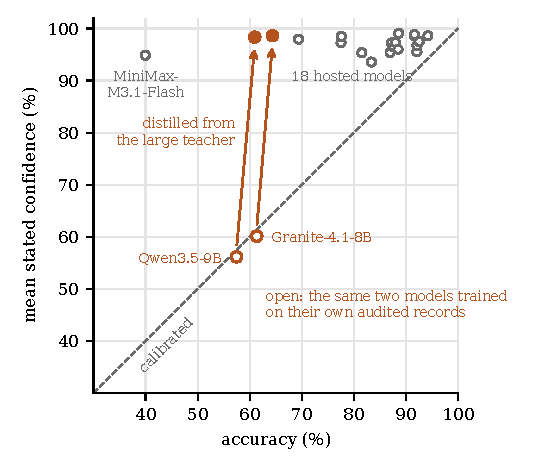
\includegraphics[width=0.5\linewidth]{fig6-dunning-kruger.pdf}
\caption{\textbf{Figure 3. Stated confidence does not fall with accuracy, and students trained on a large teacher's confidence land in the same band.} The arrows compare two training conditions of the same base model, not one model over time. Each grey circle is one of \panelIncluded{} hosted models (Table~6): accuracy (x) against mean stated confidence (y) on the 1{,}000 evaluation questions; on the dashed line the two are equal. Open orange circles: Qwen3.5-9B and Granite-4.1-8B trained on their own audited records; filled: the same base models trained on DeepSeek-V4.1-Flash answers with the teacher's own confidence. Greedy answer for all models, seed 1 for the students; hosted models were served by a provider and ran under one prompt (Appendix A, Responsible use). Source: \texttt{paper/figures.py} $\to$ \texttt{results/panel.json}, \texttt{results/dist\_cells.json}.}
\end{figure}

\begin{figure}[h]
\centering
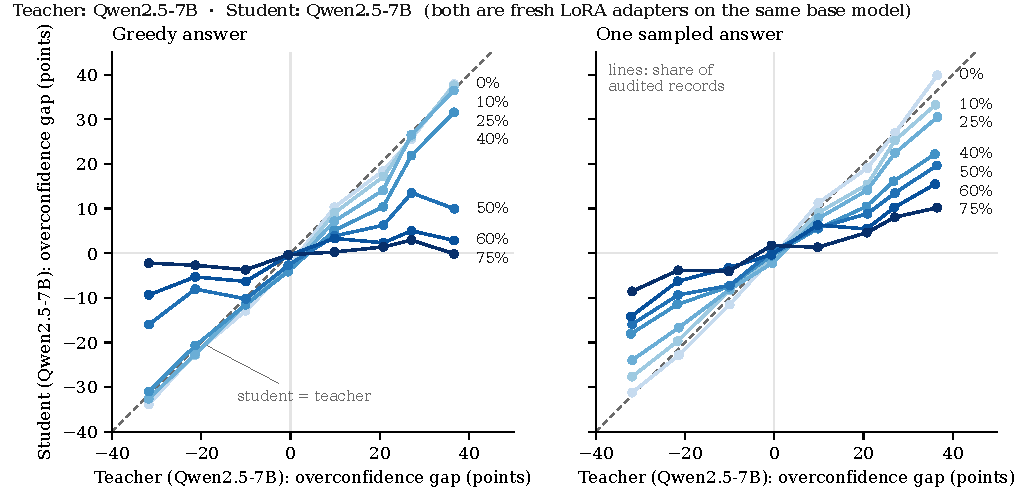
\includegraphics[width=0.6\linewidth]{fig1-return-map.pdf}
\caption{\textbf{Figure 8. A student inherits its teacher's overconfidence; unmarked audits reach the sampled answer in proportion and the greedy answer mainly between 40\% and 60\%.} Teacher and student are both Qwen2.5-7B (separate adapters on the same base model). Each point is one student, placed by its teacher's gap (x) and its own (y) on 1{,}000 held-out questions; lines connect students with the same share of audited records. Left: greedy answer. Right: one sampled answer per question. Source: \texttt{paper/figures.py} $\to$ \texttt{results/runs.json}.}
\end{figure}

\begin{figure}[h]
\centering
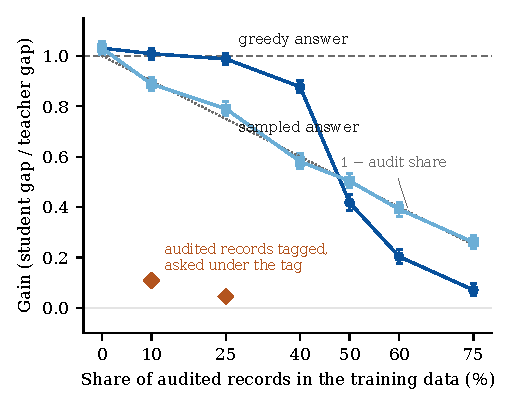
\includegraphics[width=0.64\linewidth]{fig2-gain.pdf}
\caption{\textbf{Figure 6. The same audits, two readouts.} Teacher and student are both Qwen2.5-7B. Left: gain against audit share; the sampled answer follows one minus the audit share, the greedy answer holds near one and drops between 40\% and 60\%. Diamonds: audited records carried a tag and the model was asked under it. Bars: 95\% bootstrap intervals. Right: weight of audit-style confidence values in the student's replies (mean over eight teachers; bars: lowest and highest teacher). Source: \texttt{paper/figures.py} $\to$ \texttt{results/summary.json}.}
\end{figure}

\begin{figure}[h]
\centering
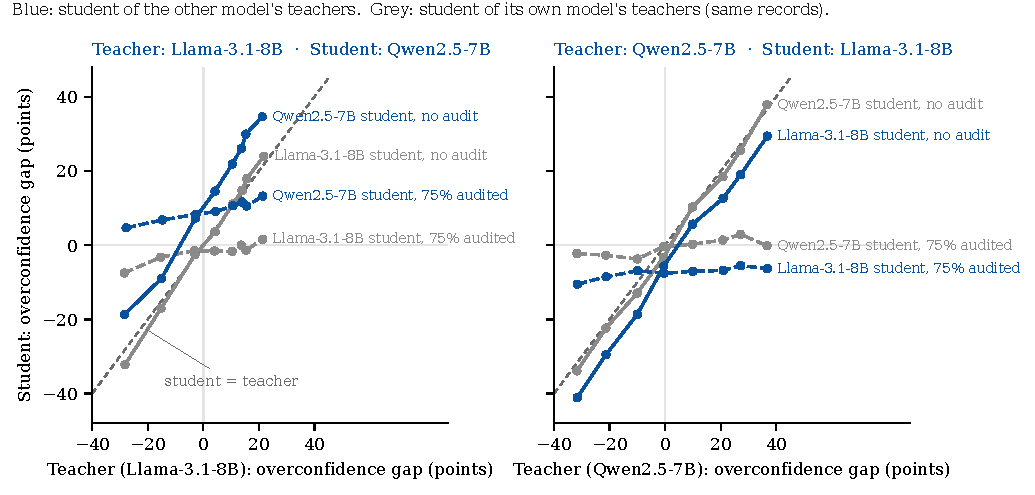
\includegraphics[width=0.56\linewidth]{fig5-cross-family.pdf}
\caption{\textbf{Figure 7. Between two older models: confidence transfers, calibration does not.} Blue: students of the other model's teachers; grey: students of their own model's teachers, same records. Solid: no audit; dashed: 75\% audited. Greedy answer; x is the teacher's own gap. Left: Llama-3.1-8B teachers (70\% accurate), Qwen2.5-7B students (57--59\%). Right: the reverse. Source: \texttt{paper/figures.py} $\to$ \texttt{results/summary*.json}.}
\end{figure}

\begin{table}[h]
\centering\small
\caption{\textbf{Table 1. Does a starting gap survive four generations?} Qwen2.5-7B. Each cell: overconfidence gap of the greedy answer / of the sampled answer, in points. Generation 0 is the installed teacher (its sampled readout was not recorded). Arms: no audit; 25\% audited with sampled records; 25\% audited with greedy records. One run per cell; seed noise is about \seedSD{} point.}
\tableChain
\end{table}

\begin{table}[h]
\centering\small
\caption{\textbf{Table 2. How much of the teacher's gap reaches the student?} Gain = slope of student gap on teacher gap across eight teachers (95\% bootstrap interval). 1 = unit slope, 0 = student gap independent of teacher gap; intervals are question-bootstrap intervals with models fixed. Columns are the two readouts. Last four rows: audited records carried a tag and the model was asked under the ``verified'' or ``unverified'' tag (seven teachers).}
\tableGain
\end{table}

\begin{table}[h]
\centering\small
\caption{\textbf{Table 3. Does the one-generation map forecast four generations?} Map fitted on installed teachers and their students, iterated four times from the chain's start; sampled-records arm. Error = observed minus predicted at generation 4, joint question-bootstrap interval with models fixed. Gaps in points.}
\tableForecast
\end{table}

\begin{table}[h]
\centering\small
\caption{\textbf{Table 4. Every cell of the return map, greedy answer.} Student overconfidence gap in points by teacher gap (rows) and audit share (columns).}
\tableMapGreedy
\end{table}

\begin{table}[h]
\centering\small
\caption{\textbf{Table 5. Every cell of the return map, sampled answer.} Same layout.}
\tableMapSampled
\end{table}

\begin{figure}[h]
\centering
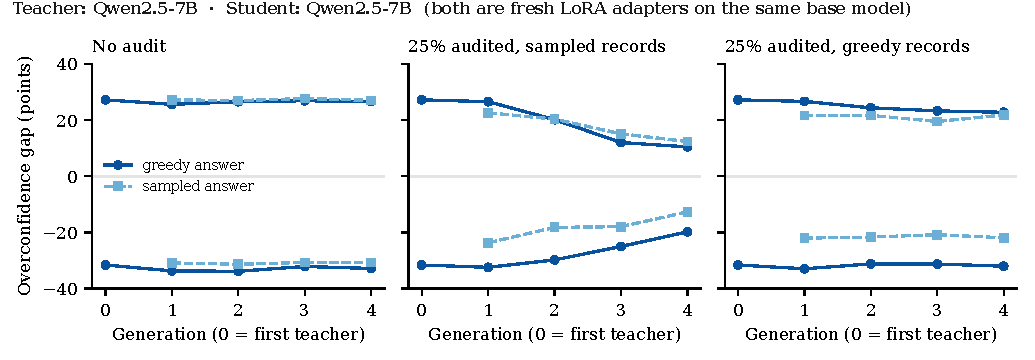
\includegraphics[width=\linewidth]{fig3-chains.pdf}
\caption{\textbf{Figure 4. Chains of four generations.} Teacher and student are both Qwen2.5-7B. Overconfidence gap per generation from the most over- and underconfident teacher, in three arms. Numbers in Table~1. Source: \texttt{paper/figures.py} $\to$ \texttt{results/summary.json}.}
\end{figure}

\begin{table}[h]
\centering\small
\caption{\textbf{Table 6. Hosted models on the same questions.} Accuracy and stated confidence in \%, gap in points. Models with fewer than 90\% of replies in format are excluded: \panelExcluded{}.}
\tablePanel
\end{table}

\llamaAppendix{}

\newAppendix{}

\section*{Appendix D. Author Contributions and Acknowledgements}
Martin Kaiser chose the direction (the Forethought feedback-loop claim, overconfidence as the trait, the interest in tiered treatment of data), chose the three follow-up arms from a list of candidates, asked for a third, newer model family (Qwen3-8B), judged that the copying result alone was expected mechanics and asked for the distillation test with a larger teacher, required current models for it in place of models chosen for comparability with the earlier runs, set the budget and reviewed the results. See the LLM usage statement for what the AI assistant did.

\textbf{Acknowledgements.} All compute and API use ran on free credits: Modal (GPU training and evaluation), Nebius Token Factory (hosted-model panel, the teachers of the distillation arm and the Qwen3-235B scorer check; credits offered to Apart Research sprint participants), Anthropic (Claude Haiku 5.5 scorer check and Claude Code as research assistant) and OpenAI (Codex reviews of drafts and plan). Models and TriviaQA were downloaded from Hugging Face. We thank Apart Research for organising the sprint.

\section*{LLM Usage Statement}
An AI assistant (Claude, in Claude Code) proposed the candidate ideas, wrote the protocol, the code and the analysis, launched and monitored the runs, produced the figures and drafted this report; a second assistant (OpenAI Codex) reviewed drafts and the plan. Martin Kaiser chose among the ideas, pointed to the Forethought essay, chose overconfidence as the trait, set the budget, and reviewed the design and results. Every number in the report is generated by script from the public result files.

\end{document}
